\section{Обзор архитектуры DaVinci}
\label{sec:Chapter6} \index{Chapter6}

\subsubsection{Общее описание}

Архитектура DaVinci --- нейропроцессор (NPU, neural processing unit),
разработанный компаней HiSilicon (подразделение Huawei). В отличие от
обычных CPU и GPU, которые необходимы для вычислений общего назначения,
и ASIC, предназначенной для конкретного алгоритма, архитектура Da Vinci
предназначена для исполнения уже обученных нейронных сетей. Работа с NPU
является обычной схемой гетерогенных вычислений, в ней CPU является хостом
(главным устройством, которое запрашивает вычисления), а NPU --- девайсом
(подчинённым устройством, производящим вычиления). Взаимодействие между ними
происходят по следующему алгоритму:

\begin{enumerate}
    \item Хост производит инициализацию, необходимую для общения с девайсом.
    \item Хост аллоцирует память (общую для него и девайса) и загружает данные в неё.
    \item Хост загружает объектный файл девайса и регистрирует функцию для исполнения.
    \item Хост передаёт указатели на аллоцированную память и даёт команду к исполнению.
    \item Девайс исполняет выбранную функцию.
    \item Хост копирует результат исполнения девайса к себе.
\end{enumerate}

Процессоры, основанные на архитектуре DaVinci и их основные характеристики
представлены в таблице ниже:

\begin{table}[h!]
    \centering
    \begin{tabular}{|c|c|c|c|c|}
        \hline
        Процессор & Производительность для float 16/int 8 & Мощность & Тех. процесс  \\ \hline
        Ascend 910 & 320/640~терафлопс & 310~Вт & 7~нм, N7+ \\ \hline
        Ascend 310 & 16/8~терафлопс & 8~Вт & 12~нм, FFC \\ \hline
    \end{tabular}
\end{table}

Теперь перейдём к внутреннему устройствую чипа Ascend. Схема архитектуры
представлена на рисунке. Рассмотрим её основные особенности.

\begin{figure}[h!]
    \centering
    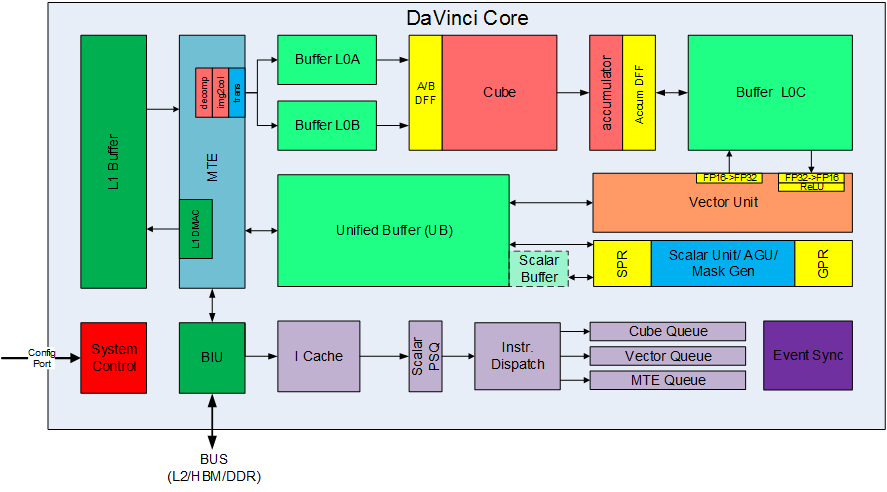
\includegraphics[scale=0.5]{DaVinci.png}
    \caption{Архитектура DaVinci}
\end{figure}

В ядре есть три вычислительных юнита: матричный, векторный и скалярный,
которые используются для соответствующих вычилений.  Исполнение на юнитах
происходит параллельно, для каждого юнита существует
отдельная, независимая очередь задач. Ещё три очереди предназначены для
копирования из разных буфферов друг в друга (о них речь пойдёт ниже).
Для синхронизации очередей используются команды \texttt{set\_flag} и \texttt{wait\_flag},
которые по своей сути представляют систему событий. Первая команда сигнализирует,
что событие произошло, а вторая запускает ожидание события. Правильное
использование механизмов синхронизации позволяет значительно увеличить
загрузку всех юнитов и, следовательно, снизить общее время исполнения.
В данной работе не будут рассматривать проблемы с расстановкой операций
синхронизации и будет считаться, что они всегда расставлены наиболее
оптимальным образом.

\subsubsection{Матричный юнит}

Матричный юнит на вход принимает матрицы с типом элементов \texttt{float 16}
или \texttt{int 8}, на выходе же элементы имеют тип \texttt{float 16},
\texttt{float 32} или \texttt{int 32}. Умножение работает в двух режимах:

\begin{enumerate}
    \item Обычное умножение: $C = A \times B$
    \item Режим накопления: $C = A \times B + C$, т.~е. результат текущего
          умножения прибавляется к предыдущему.
\end{enumerate}

Каждая из входных матриц должна быть разбита на блоки $16 \times 16$
(в случае \texttt{float 16}) или $16 \times 32$ (в случае \texttt{int 8}).
Расположение элементов внутри блоков и блоков относительно друг друга также
различно. Существуют две стратегии размещения: про строкам (формат \texttt{Z})
и по столбцам (формат \texttt{N}). Примем обозначение: размещение внутри блока
обозначается строчной буквой, а между блоками --- заглавной. При умножении
матрица $A$ должна быть заранее быть записана в формате \texttt{Zz},
матрица $B$ --- в формате \texttt{Zn}, а выходная матрица $C$ будет \texttt{Nz}.

Матричный юнит работает по принципу систолического массива.
Систолический массив --- однородная сеть тесно связанных блоков обработки данных.
Его схему для архитектуры DaVinci можно увидеть на картинке ниже.

Принцип умножения довольно прост: за первый такт (FIXME: лучше не использовать
слово такт в данном контексте) происходят все умножения,
после чего за оставшиеся четыре такта произведения суммируются. Таким
образом, за пять тактов можно перемножить две матрицы \texttt{16x16}.
Матричный юнит, итерируясь по матрицам и перемножая их поблочно, быстро
получает результат перемножения.

\begin{figure}[h!]
    \centering
    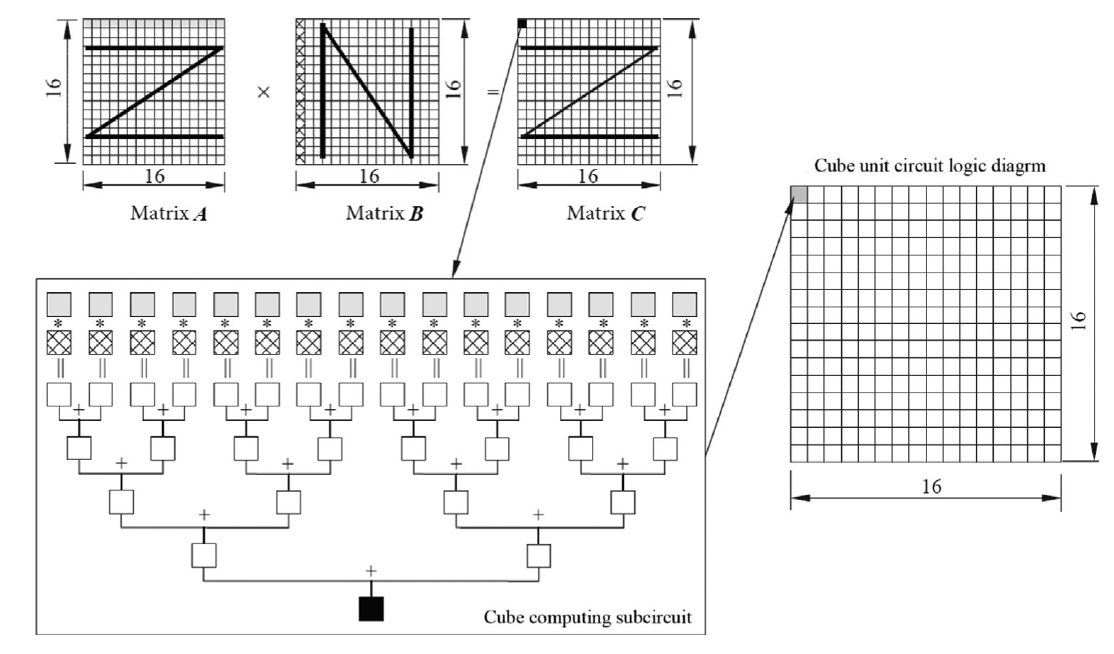
\includegraphics[scale=0.5]{Systolic.png}
    \caption{Схема вычисления в матричном юните}
\end{figure}

\subsubsection{Векторный юнит}

Теперь рассмотрим работу векторного юнита. Существуют два режима работы:
\textit{common} и \textit{VA}. В обоих случаях память делится на блоки
по 32 байта, а векторная операция представляется в виде цикла, на каждой
итерации которого обрабатывается 8 блоков. Таким образом, за одну итерацию
может быть обработано 128 элементов типа \texttt{float 16} или 64 элемента
32-разрядных типов (\texttt{float 32}, \texttt{int 32}). Стоит отметить, что
не обязательно обрабатывать такое количество элементов. Для выбора, с какими
именно элементами будет работать операция необходимо задать маску. Векторный
юнит обрабатывает только те элементы, на позиции которых в маске стоит бит 1.
На каждой следующей итерации блоки сдигаются на заранее заданный шаг,
после чего операция повторяется. Отличаются режимы способом описания этих блоков.
В случае \textit{VA} режима блоки задаются в виде восьми указатей, а в случае
\textit{common} --- указателем на первый блок и шагом между блоками. Для первого,
второго аргумента и результата шаг может быть различным. 
Юнит поддерживает большое количество операций: математических, логических,
приведения типов и т.~д. Есть и спецефичные операции: \textit{relu}, часто
используемый в нейронных сетях, операция транспонирования.

\subsubsection{Память}

Память ядра неоднородна. В ядре существует 5 буферов:
L1, L0A, L0B, L0C, UB. Также существует внешняя память (GM), через которую
происходит общение с хостом. Опишем общую схему потока данных между этими кэшами.
Данные из внешней памяти загружаются в L1 и UB. Данные в UB предназначены для
обработки векторным и скалярным юнитами. Данные из L1 загружаются в L0A и L0B,
которые соответствуют матрицам A и B матричного умножения. Результат после
перемножения (которое, как было упомянуто раньше, выполняется матричным юнитом),
попадает в буфер L0C, из которого происходит данные отправляются в UB. Выгрузка
результата вычислений во внешнюю память возможна только из UB. Отметим, что
описанные выше буферы имеют небольшой размер, что является одной из основных
проблематик нашей работы. Более подробно этот вопрос будет рассмотрен в главе,
посвященной ловерингу.

\subsubsection{Свёртка}

Реализация свёртки на нейроматрицных процессоров несколько сложнее, чем умножения.
На некоторых архитектурах (FIXME: ссылка) она поддержана нативно. К сожалению, наша
не является таковой. Но с помощью особого преобразования её можно свести к 
умножению матриц. Приведём некоторые общие соображения, которые позволят понять его.

Итак, пусть есть входное изображение (\textit{image}) размеров $H_i \times W_i$,
содержащее $C$ цветов. Будем называть его \textit{входной картой признаков}
(\textit{input feature map}). Ядро (\textit{kernel}) свёртки представляет из
себя небольшую матрицу размеров $H_k \times W_k$ (характерный размер --- $3-5$).
Ядро имеет такое же количество входных цветов $C$, но также имеет и $F$
выходных цветов. Таким образом, изображение имеет формат $H_i W_i C$,
а ядро --- $F H_k W_k C$. Выходная карта признаков, имеет структуру, схожую
со входной: $H_o W_o F$, где $H_o = H_i - H_k + 1$, $W_o = W_i - W_k + 1$
в простейшем случае. Если обозначить: $a$ --- входная карта, $k$ --- ядро,
$c$ --- выходная, то свёрка выражается следующей формулой:

\[
    c_{ijf} = \sum \limits_{h = 0}^{H_k} \sum \limits_{w = 0}^{W_k}
              \sum \limits_{c = 0}^{C} a_{i+h, j+w, c} \cdot k_{f h w c}
\]

Заметим, что операция чем-то схожа на скалярное умножение векторов
(если цвета считать вектором) или матричное умножение. Если первый тензор
преобразовать в матрицу $A$, где одной строке будет соответвовать одна
такая сумма (т.е. размеры матрицы станут $H_o W_o \times H_k W_k C$), а
ядро --- в матрицу $K$ размеров $H_k W_k C \times F$, то выходная
матрица $C = A \times K$. Этот процесс преобразования входной карты
признаков называется \textit{img2col} (\textit{image-to-column}),
оно содержится в архитектуре команд целевого процессора.

Таким образом, свёрка есть композиция \textit{img2col} и умножения матриц.
Отметим, что в реальности свёртка имеет такие параметры, как
\textit{stride}, \textit{dilation} и \textit{pad}. Они усложняют
приведённые формулы, но не меняют сути происходящего. Также в
качестве обобщения можно взять $N$ изображений, форматы входной и
выходной карт приобретают вид $N H_i W_i C$ и $N H_o W_o F$ соответственно.


\newpage
